\documentclass[document.tex]{subfiles}
\begin{document}
\section*{Exercise 4:}


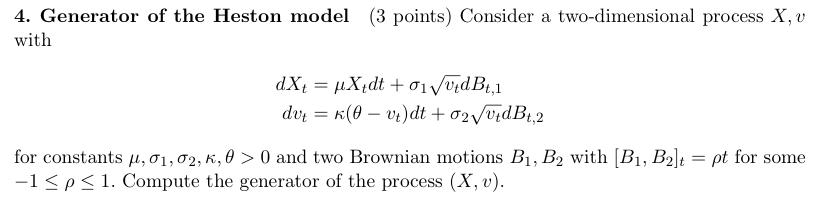
\includegraphics[width=\textwidth]{ex4.png}


\begin{align*}
Af(t,x)=\sum_{i=1}^{n} \mu_i(t,x) \frac{\partial f}{\partial x_i} (x) + \frac{1}{2} \sum_{i,j=1}^n c_{ij} (t,x) 
\frac{\partial^2 f}{\partial x_i \partial x_j} (t,x)
\end{align*}

In our case the generator of (X, v) is given by:
\begin{equation}
Af(t, X, v) = \mu_X(t, X, v)^t \Delta f + \frac{1}{2} C_{XX} f_{XX} + C_{Xv} f_{Xv}(t, X, v) + \frac{1}{2} C_{vv} f_{vv}
\end{equation}

$\mu$ is given by the deterministic part of the stochastic process:
\begin{equation}
\mu(t, X, v) = (\mu X_s dt, \kappa (\theta - v_s) dt)^t
\end{equation}


We get the variance term by:
\begin{equation}
\sigma(t, X, v) = (\sigma_1 \sqrt{v_s} d B_1, \sigma_2 \sqrt{v_s} d B_2)^t
\end{equation}
\begin{equation}
C(t, X, v) = \sigma(t, X, v) \sigma(t, X, v)^t
\end{equation}

\begin{equation}
C(t, X, v)_{XX} = \sigma_1^2 v_s d [B_1, B_1] = \sigma_1^2 v_s d t
\end{equation}
\begin{equation}
C(t, X, v)_{vv} = \sigma_2^2 v_s d [B_2, B_2] = \sigma_2^2 v_s d t
\end{equation}

We know:
\begin{equation}
[B_1, B_2]_t = \rho
\end{equation}
\begin{equation}
C(t, X, v)_{Xv} = C(t, X, v)_{vX} = \sigma_1 \sigma_2 v_s d [B_1, B_2] = \sigma_1 \sigma_2 v_s \rho d t
\end{equation}

We use this to rewrite the very first expression as:
\begin{equation}
Af(t, X, v) = \mu X_t f_X + \kappa (\theta - v_t) f_v + \frac{1}{2} \sigma_1^2 v_t f_{XX} + \sigma_1 \sigma_2 v_t \rho f_{Xv} + \frac{1}{2} \sigma_2^2 v_t f_{vv}
\end{equation}

\end{document}
